\documentclass[12pt,a4paper]{article}
\usepackage[utf8]{inputenc}
\usepackage[english]{babel}
\usepackage{graphicx}
\usepackage{amsmath}
\usepackage{amssymb}
\usepackage{geometry}
\usepackage{hyperref}
\usepackage{listings}
\usepackage{xcolor}
\usepackage{fancyhdr}
\usepackage[none]{hyphenat}
\usepackage{float}
\usepackage{enumitem}
\usepackage{titlesec}
\usepackage{tikz}
\usepackage{setspace} % For line spacing
\usepackage{times} % For Times New Roman font
\usepackage{algorithm}
\usepackage{algpseudocode}
\usepackage{algorithmicx}
\usepackage{csquotes}
\usepackage{xurl}  % Pentru URL breaking
\usepackage{url}   % Pentru text breaking
\usepackage{seqsplit} % Pentru împărțirea automată a textului lung
\usepackage[backend=biber, style=numeric, sorting=ynt]{biblatex}
\addbibresource{bibliografie.bib}

\usetikzlibrary{arrows.meta, positioning, shapes.geometric}

% Comandă pentru cod care se poate întrerupe
\newcommand{\code}[1]{\texttt{\detokenize{#1}}}
\newcommand{\breakablecode}[1]{\url{#1}}

% Redefinire \texttt pentru a permite întreruperea automată
\let\oldtexttt\texttt
\renewcommand{\texttt}[1]{%
    \oldtexttt{\seqsplit{#1}}%
}


% Remove redundancies and warnings

\geometry{
    a4paper,
    top=2.5cm,
    bottom=2.5cm,
    left=2.5cm,
    right=2.5cm
}

\hypersetup{
    colorlinks=true,
    linkcolor=blue,
    filecolor=magenta,      
    urlcolor=cyan,
}

% Code styles
\definecolor{codegreen}{rgb}{0,0.6,0}
\definecolor{codegray}{rgb}{0.5,0.5,0.5}
\definecolor{codepurple}{rgb}{0.58,0,0.82}
\definecolor{backcolour}{rgb}{0.95,0.95,0.92}

\lstdefinestyle{mystyle}{
    backgroundcolor=\color{backcolour},   
    commentstyle=\color{codegreen},
    keywordstyle=\color{magenta},
    numberstyle=\tiny\color{codegray},
    stringstyle=\color{codepurple},
    basicstyle=\ttfamily\footnotesize,
    breakatwhitespace=false,         
    breaklines=true,                 
    captionpos=b,                    
    keepspaces=true,                 
    numbers=left,                    
    numbersep=5pt,                  
    showspaces=false,                
    showstringspaces=false,
    showtabs=false,                  
    tabsize=2
}

\lstset{style=mystyle}


% Text configuration
\setstretch{1.5} % Line spacing
\setlength{\parindent}{0pt} % Remove paragraph indentation
\setlength{\parskip}{6pt} % Space between paragraphs


\begin{document}

\begin{titlepage}
    \centering
    \begin{tabular}{p{2.5cm}p{10cm}p{2.5cm}}
    \includegraphics[width=2.5cm]{screenshots/s8.png} & 
    \begin{center}
    \vspace{-3.2cm}
    \textbf{Department of Automatic Control and Industrial Informatics}\\
    \textbf{Faculty of Automatic Control and Computers}\\
    \textbf{National University of Science and Technology}\\
    \textbf{POLITEHNICA Bucharest}\\
    Splaiul Independenţei 313, 060042, Bucharest, Romania\\
    Room ED 412, Tel. 021/402.92.69\\
    \href{http://www.aii.pub.ro}{www.aii.pub.ro}, email: secretariat.aii@upb.ro
    \end{center} & 
    \includegraphics[width=2.5cm]{screenshots/s9.png} \\
    \end{tabular}
    
    \vspace{3cm}
    
    {\Large\bfseries\centering Student Scientific Communications Session}

    {\large\bfseries\centering 2025 Edition}

    \vspace{2cm}
    
    {\LARGE\bfseries\centering Anti-Plagiarism Monitoring System for Exams\\[2cm]}

    \vspace{\fill}
    
    \raggedright
    {\large\bfseries Author: Valentin PLETEA-MARINESCU, Faculty of Automatic Control and
    Computers, 3rd year, Group 332AB \par}
    {\large\bfseries Email address: pletea.valentin2003@gmail.com \par}
    {\large\bfseries Scientific advisor: Assoc. Prof. Dr. Eng. Ștefan Alexandru MOCANU\par}
\end{titlepage}

\hypersetup{linkcolor=black}
\tableofcontents
\newpage

\section{Introduction}

\subsection{Context and relevance of the topic}

Plagiarism represents one of the serious problems of the educational system, and since the emergence and development of artificial intelligence, things have intensified. The choice of this topic consists in the opportunity to offer equal chances to all participants in an exam, and this anti-plagiarism system, proposed in this project, represents an innovative solution, through the combination of modern image processing techniques and artificial intelligence\cite{russell2020artificial}, which aims to monitor the behavior of candidates and signal possible fraud attempts.

The use of mobile phones as an instrument of cheating in examination halls has increased
considerably in recent years, creating an additional burden on supervisors in ensuring
exam integrity\cite{nazari2019detection}. Moreover, recent studies in the field of academic integrity show that plagiarism is "an ethical deviation that affects the quality, legibility and
credibility" of academic results, being essential the development of solutions to combat
unacceptable practices\cite{zimba2021plagiarism}.

According to the study conducted by Gabriela Pelican\cite{pelican2021plagiat}, plagiarism
affects absolutely all educational levels, and in the case of
Romania, things are not going very well in this regard, the author
mentioning that "Romania presents the highest rate of plagiarism
discovered in the Union territory, namely 26.1\% of all
verified works, a value almost double compared to the European
average, as well as the fact that the incidence of plagiarism cases is
much higher in the countries of the eastern region of Europe, countries whose
living and education levels are considerably lower
compared to western countries."

Also, another study\cite{brainard2018massive}, published by Science, tells us that Romania is the country with the highest number of
scientific articles removed from the content of specialized publications as
a result of non-compliance with conduct standards in scientific research,
by reporting to the total funds allocated for research and
also, it ranks second in the ranking of countries with the highest number of
withdrawn articles relative to the total articles published, following
the discovery of plagiarism.

\newpage

\subsection{Project objectives}

This project aims to provide an innovative system for exam monitoring, with the following specific objectives:

\begin{enumerate}[label=\arabic*.]
    \item \textbf{Candidate gaze detection:} Signaling and recording situations
    where the candidate looks in other directions such as left, right or down, 
    rather than at their own monitor screen or at their own sheet, in the case of a written exam.
    
    \item \textbf{Identification of unauthorized objects:} Detection of devices such as
    smart watches or phones, which can be used to obtain information, 
    which would lead to fraud of the respective exam.
    
    \item \textbf{Recording and archiving:} Creating a video recording in which 
    exam sessions will be captured and archived for subsequent analysis, 
    highlighting probable fraud attempts.
    
    \item \textbf{Report generation:} Creating detailed reports in HTML, CSV and JSON formats,
    thus contributing to a clearer and safer analysis for evaluators.
    
    \item \textbf{Intuitive interface:} Development of an intuitive graphical interface that allows
    supervisors to use all the functionalities mentioned above.
\end{enumerate}

\subsection{Advantages of the proposed approach}

In general, many anti-plagiarism solutions focus more 
on monitoring the candidate's screen, but this system is centered on 
their physical behavior. I believe that by tracking the direction of gaze 
and detecting unauthorized objects, the system can identify clues of
fraudulent behavior, providing concrete evidence that can be analyzed later. 
This can contribute significantly to maintaining academic integrity, 
without the need to create that atmosphere of excessive surveillance.

It is normal for the respective system to offer, in addition to
remarkable results, false positives as well, due to factors such as
the illumination of the exam room or natural head movements, without
the intention of looking in another direction. Thus, through the
video recording and real-time signaling functionalities of
possibly fraudulent behaviors, there can be, after the completion of
the respective exam, a discussion between teacher and student based on
their honesty to reach the final result.

Technology advances day by day, and various plagiarism attempts automatically diversify.
Therefore, it is absolutely natural that the systems that try, through
various means, to combat exam fraud, also advance.

\section{Domain analysis and existing solutions}

\subsection{Similar existing solutions on the market}

Various monitoring and anti-fraud solutions have appeared on the market over time for exams. Following research, I identified
three main systems that propose solutions similar to this project: ProctorU\cite{proctoru}, 
Proctorio\cite{proctorio} and Respondus Lockdown Browser\cite{respondus}.

Recently, modern online surveillance systems like Honorlock have implemented advanced technologies 
that detect mobile phone use "through a combination of surveillance tools" and can
determine when participants attempt to use unauthorized mobile devices to access 
content during exams\cite{honorlock2023detecting}. Also, recent research in the field of 
eye-tracking has proposed "a new solution for detecting cheating in online exams using 
gaze tracking technology"\cite{dilini2021cheating}, demonstrating the effectiveness of this approach
in detecting suspicious behavior.

\subsubsection{ProctorU}
ProctorU is one of the most used platforms in
online exam supervision. It is based both on monitoring
the candidate's screen and their behavior. 

\begin{table}[h]
\centering
\begin{tabular}{|p{7.5cm}|p{7.5cm}|}
\hline
\textbf{Strengths} & \textbf{Limitations} \\
\hline
\begin{itemize}
    \item Candidate identity verification through ID or identity document
    \item Real-time human supervision
    \item Complete monitoring of computer activity
    \item Suspicious behavior detection through AI
\end{itemize} & 
\begin{itemize}
    \item High costs (15-25 USD per candidate)
    \item Requires stable internet connection
    \item Less suitable for physical exams
    \item Potential privacy issues
\end{itemize} \\
\hline
\end{tabular}
\caption{Comparative analysis of the ProctorU system}
\end{table}

\newpage

The platform records every second, ensures that no other tabs are
open, except the one in which the respective exam is taken,
does not allow certain keyboard combinations for functions like 
print, copy or paste and, through a webcam, the platform can 
efficiently supervise the candidate.

\subsubsection{Proctorio}
Another similar system is Proctorio, similar to
ProctorU, but which is completely automated, as it relies only
on AI and machine learning technologies for detecting possible
fraud attempts, without the need for human assistance.

\begin{table}[H]
\centering
\begin{tabular}{|p{7.5cm}|p{7.5cm}|}
\hline
\textbf{Strengths} & \textbf{Limitations} \\
\hline
\begin{itemize}
    \item Simple installation and configuration through browser extension
    \item Web browsing blocking functionalities
    \item Algorithms that reduce the need for human intervention
    \item Lower costs than ProctorU
\end{itemize} & 
\begin{itemize}
    \item High rate of false positives
    \item Difficulty in detecting secondary device use
    \item Works only on Google Chrome
    \item Privacy issues
\end{itemize} \\
\hline
\end{tabular}
\caption{Comparative analysis of the Proctorio system}
\end{table}

Monitoring is based on facial recognition, analyzing behavior through 
head or eye movement. The system also handles screen monitoring, observes if other tabs are open and if background applications are running that could facilitate exam fraud.

\subsubsection{Respondus Lockdown Browser}
Respondus Lockdown Browser represents a different approach, 
as it focuses on creating a secure exam environment,
by blocking the candidate's access to other applications and resources.

According to its official documentation\cite{respondus}, this solution
integrates with learning management systems (LMS), such as Canvas,
Blackboard, Moodle, Schoology and Brightspace.

\begin{table}[H]
    \centering
    \begin{tabular}{|p{7.5cm}|p{7.5cm}|}
    \hline
    \textbf{Strengths} & \textbf{Limitations} \\
    \hline
    \begin{itemize}
        \item Prevents access to other programs and resources
        \item Good integration with educational platforms (LMS)
        \item Lower costs compared to other solutions
        \item Easy to implement at institutional level
    \end{itemize} & 
    \begin{itemize}
        \item Inability to detect secondary devices
        \item Does not monitor candidate's physical behavior
        \item Limited functionality on mobile devices
        \item Incompatibility with specific programs (IDEs, etc.)
    \end{itemize} \\
    \hline
    \end{tabular}
    \caption{Comparative analysis of the Respondus Lockdown Browser system}
\end{table}

\subsection{Relevant multimedia aspects}

\subsubsection{Protocols and data transmission}
In terms of multimedia-related aspects, we encounter protocols that
ensure secure and optimized data transmission:
\begin{itemize}
    \item \textbf{WebRTC} for real-time audio-video communication. This protocol is used to transmit the video stream captured from the webcam to the processing system, ensuring minimal latency and optimal transmission quality\cite{sredojev2015webrtc}. In our project, WebRTC is used to enable real-time candidate monitoring, providing a stable and efficient connection.
    \item \textbf{TLS/SSL} for encrypting the entire data stream. This security layer is essential to protect data transmitted between client and server, preventing unauthorized access or interception of sensitive information\cite{yang2018tls}. In the context of our project, TLS/SSL is used to secure both the video stream and the generated data, such as violation reports.

    Although the current version of our project is based on local processing without network communication components, implementing these technologies would represent a valuable direction for future development, allowing remote monitoring of candidates.
\end{itemize}

\subsubsection{Video processing}
Regarding video processing, the stream captured from the webcam is processed in real time to detect suspicious behavior. For saving recordings, our system uses standard formats like MP4, which incorporates the H.264 codec, ensuring good efficiency in storage space usage\cite{goodfellow2016deep}.

Recent research in the field of exam surveillance systems has demonstrated the effectiveness of facial detection and eye tracking for identifying suspicious behavior\cite{alem2021novel}. Our implementation is based on these studies, integrating libraries like \texttt{dlib} and \texttt{OpenCV} to detect face position and gaze direction, thus providing a robust solution for identifying suspicious behavior.

This system focuses primarily on visual analysis, detecting both the candidate's gaze direction and the presence of unauthorized objects such as mobile phones and smart watches, elements that represent the most frequent means of exam fraud.

\subsubsection{Watermarking}
In Lockdown Browser type solutions, visible or invisible watermarks are applied over the content displayed on the screen, with the purpose of preventing unauthorized capture of exam information. In our project, watermarks are used to mark the recorded video stream with information such as the real date and time, but also the H and V values, which indicate the limits within which the candidate's gaze direction is found. This type of marking contributes to ensuring the authenticity and integrity of recorded data.

\subsubsection{Event synchronization}
To ensure precise correlation between video frames and detected events, our project uses temporal markings. These are generated at the moment of capturing each video frame and are used to link the alerts generated by the system with the exact moment of the violation. This approach allows subsequent consultation of video recordings and efficient verification of generated reports, thus providing concrete evidence for evaluating the candidate's behavior during the exam.

\subsubsection{Optimizations for limited resources}
To enable efficient system operation on devices with limited resources, several optimizations have been implemented in this system:
\begin{itemize}
    \item Processing one frame out of 30 for object detection, thus reducing resource consumption.
    \item Using a circular buffer for efficient video frame management.
    \item Integrating a cache system for generated alerts, avoiding duplication of alert messages.
\end{itemize}

\subsection{Advantages of the proposed solution compared to existing ones}

The anti-plagiarism monitoring system developed within this project offers numerous comparative benefits compared to alternatives currently available on the market:

\begin{enumerate}
    \item \textbf{Complete physical behavior monitoring} - While most commercial solutions (such as Proctorio or Respondus) are limited to supervising activity on the computer screen, our system observes the candidate's movements and gestures. This approach allows detection of fraud tactics that would otherwise go unnoticed, such as consulting physical notes or communicating with other people through gestures. The system analyzes gaze direction, head orientation and other physical clues that may signal fraudulent intentions.
    
    \item \textbf{Precise identification of unauthorized electronic devices} - Through implementation of YOLOv8 algorithms and modern object recognition techniques, our application can identify with high accuracy mobile phones, smart watches and other devices frequently used for cheating. This capability significantly exceeds the functionalities offered by Respondus Lockdown Browser, which cannot detect secondary device use, and even those of ProctorU, which relies heavily on human supervisors for this task.
    
    \item \textbf{Advanced reporting and documentation system} - The application automatically generates detailed reports in versatile formats (HTML for easy viewing, CSV for Excel analysis and JSON for integration with other systems). These reports include screenshots of suspicious moments, precise time stamps and clear descriptions of incidents, providing evaluators with all necessary information to make documented decisions. The system thus maintains a complete history of the examination session, allowing subsequent verification and reducing disputes related to possible sanctions.
    
    \item \textbf{Technological independence and implementation flexibility} - This system functions as an independent application, without being constrained by the specific limitations of web browsers or online platforms. This autonomous architecture eliminates external dependencies and simplifies the installation and configuration process at the institutional level. Its independent nature allows use on a wide range of devices and operating systems, offering educational institutions the freedom to implement the solution without being forced to adopt additional technologies or services. System flexibility facilitates rapid adaptation to the specific requirements of different types of exams and academic contexts.
    
    \item \textbf{Economic efficiency and scalability} - Local system implementation offers significant advantages from a long-term cost perspective. While many existing commercial solutions operate on a per-student per-exam pricing model, which can become prohibitive for institutions with large numbers of students or frequent exams, this proposed anti-plagiarism system requires only the initial investment in existing hardware infrastructure. This scalable model allows educational institutions to monitor an unlimited number of exams without additional costs, reducing the effective cost per student with each organized session, and this approach makes anti-plagiarism monitoring technology accessible even to institutions with limited financial resources.
    
    \item \textbf{Enhanced student data confidentiality} - Through local information processing, this prototype eliminates the risks associated with transmitting data to external servers. This aspect is particularly important in the context of strict regulations regarding personal data protection, offering institutions complete control over sensitive information collected during exams.
\end{enumerate}

The combination of these advantages makes this anti-plagiarism system prototype represent an innovative and efficient solution for ensuring academic integrity, adapted to the current needs of educational institutions.

\section{Anti-plagiarism system architecture}

The developed anti-plagiarism system represents a complex software solution designed for monitoring candidates during exams, with the purpose of detecting and preventing fraudulent behavior. The system architecture was conceived according to modern software engineering principles, emphasizing modularity, extensibility and clear separation of responsibilities.

The basis of system development is represented by object-oriented programming, which allowed structuring the application into interconnected components, each having a well-defined role in the monitoring process. This approach facilitates not only the independent development and testing of modules, but also the subsequent extension of functionalities through the addition of new components.

The system processes video images as they are captured, tracking where candidates are looking and identifying unauthorized objects such as mobile phones and smart watches. This tracking is based on computer programs that can "see" and "understand" images, organized in a layered structure that keeps simple functions separate from more advanced ones.

To illustrate the system structure and operation, I have developed three complementary UML diagrams: the class diagram, the sequence diagram and the activity diagram. These representations offer different perspectives on the architecture, from the static organization of classes to dynamic control and data flows.

\subsection{Class diagram}

\begin{figure}[H]
    \centering
        \hspace{-2.7cm}
        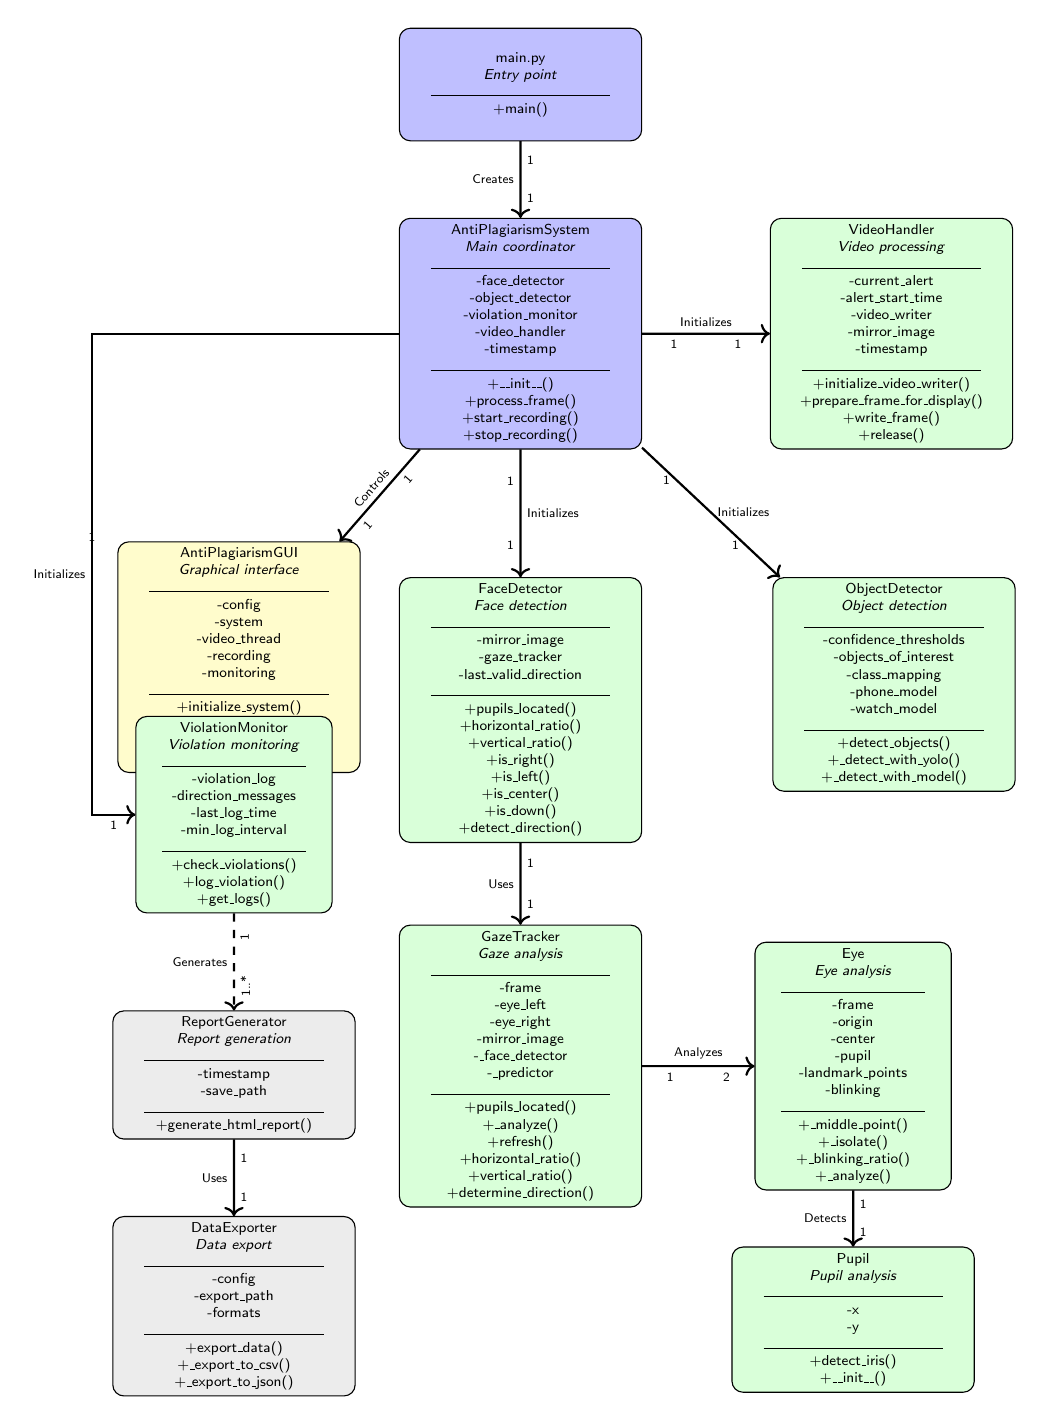
\begin{tikzpicture}[
            scale=0.65,
            transform shape,
            class/.style={rectangle, draw=black, rounded corners, text centered, text width=4.5cm, minimum height=2.2cm, font=\sffamily\footnotesize, fill=blue!10},
            smallclass/.style={rectangle, draw=black, rounded corners, text centered, text width=3.6cm, minimum height=1.8cm, font=\sffamily\footnotesize, fill=blue!10},
            mainclass/.style={rectangle, draw=black, rounded corners, text centered, text width=4.5cm, minimum height=2.2cm, font=\sffamily\footnotesize, fill=blue!25},
            uiclass/.style={rectangle, draw=black, rounded corners, text centered, text width=4.5cm, minimum height=2.2cm, font=\sffamily\footnotesize, fill=yellow!20},
            detectorclass/.style={rectangle, draw=black, rounded corners, text centered, text width=4.5cm, minimum height=2.2cm, font=\sffamily\footnotesize, fill=green!15},
            smalldetectorclass/.style={rectangle, draw=black, rounded corners, text centered, text width=3.6cm, minimum height=1.8cm, font=\sffamily\footnotesize, fill=green!15},
            utilityclass/.style={rectangle, draw=black, rounded corners, text centered, text width=4.5cm, minimum height=2.2cm, font=\sffamily\footnotesize, fill=gray!15},
            relation/.style={->, thick},
            shortrelation/.style={->, thick, shorten >=2mm, shorten <=4mm},
            aggregation/.style={->, thick},
            composition/.style={->, thick},
            dependency/.style={dashed, ->, thick}
            ]
            % Classes with attributes and methods
            \node[mainclass] (main) {main.py\\\textit{Entry point}\\\rule{3.5cm}{0.4pt}\\+main()};
            
            \node[mainclass, below=1.5cm of main] (sistem) {AntiPlagiarismSystem\\\textit{Main coordinator}\\\rule{3.5cm}{0.4pt}\\-face\_detector\\-object\_detector\\-violation\_monitor\\-video\_handler\\-timestamp\\\rule{3.5cm}{0.4pt}\\+\_\_init\_\_()\\+process\_frame()\\+start\_recording()\\+stop\_recording()};
            
            \node[uiclass, below=1.8cm of sistem, xshift=-5.5cm] (gui) {AntiPlagiarismGUI\\\textit{Graphical interface}\\\rule{3.5cm}{0.4pt}\\-config\\-system\\-video\_thread\\-recording\\-monitoring\\\rule{3.5cm}{0.4pt}\\+initialize\_system()\\+setup\_ui()\\+toggle\_monitoring()\\+toggle\_recording()};
            
            \node[detectorclass, right=2.5cm of sistem] (video) {VideoHandler\\\textit{Video processing}\\\rule{3.5cm}{0.4pt}\\-current\_alert\\-alert\_start\_time\\-video\_writer\\-mirror\_image\\-timestamp\\\rule{3.5cm}{0.4pt}\\+initialize\_video\_writer()\\+prepare\_frame\_for\_display()\\+write\_frame()\\+release()};
            
            \node[detectorclass, below right=2.5cm and -4.7cm of video] (object) {ObjectDetector\\\textit{Object detection}\\\rule{3.5cm}{0.4pt}\\-confidence\_thresholds\\-objects\_of\_interest\\-class\_mapping\\-phone\_model\\-watch\_model\\\rule{3.5cm}{0.4pt}\\+detect\_objects()\\+\_detect\_with\_yolo()\\+\_detect\_with\_model()};
            
            \node[detectorclass, below=2.5cm of sistem] (face) {FaceDetector\\\textit{Face detection}\\\rule{3.5cm}{0.4pt}\\-mirror\_image\\-gaze\_tracker\\-last\_valid\_direction\\\rule{3.5cm}{0.4pt}\\+pupils\_located()\\+horizontal\_ratio()\\+vertical\_ratio()\\+is\_right()\\+is\_left()\\+is\_center()\\+is\_down()\\+detect\_direction()};
            
            \node[detectorclass, below=1.6cm of face] (gaze) {GazeTracker\\\textit{Gaze analysis}\\\rule{3.5cm}{0.4pt}\\-frame\\-eye\_left\\-eye\_right\\-mirror\_image\\-\_face\_detector\\-\_predictor\\\rule{3.5cm}{0.4pt}\\+pupils\_located()\\+\_analyze()\\+refresh()\\+horizontal\_ratio()\\+vertical\_ratio()\\+determine\_direction()};
            
            \node[smalldetectorclass, below left=-9.6cm and 1.3cm of gaze] (violation) {ViolationMonitor\\\textit{Violation monitoring}\\\rule{2.8cm}{0.4pt}\\-violation\_log\\-direction\_messages\\-last\_log\_time\\-min\_log\_interval\\\rule{2.8cm}{0.4pt}\\+check\_violations()\\+log\_violation()\\+get\_logs()};
            
            \node[smalldetectorclass, right=1.3cm and 2.2cm of gaze] (eye) {Eye\\\textit{Eye analysis}\\\rule{2.8cm}{0.4pt}\\-frame\\-origin\\-center\\-pupil\\-landmark\_points\\-blinking\\\rule{2.8cm}{0.4pt}\\+\_middle\_point()\\+\_isolate()\\+\_blinking\_ratio()\\+\_analyze()};
            
            \node[detectorclass, below =1.1cm of eye] (pupil) {Pupil\\\textit{Pupil analysis}\\\rule{3.5cm}{0.4pt}\\-x\\-y\\\rule{3.5cm}{0.4pt}\\+detect\_iris()\\+\_\_init\_\_()};
            
            \node[utilityclass, below =1.9cm and 1.8cm of violation] (report) {ReportGenerator\\\textit{Report generation}\\\rule{3.5cm}{0.4pt}\\-timestamp\\-save\_path\\\rule{3.5cm}{0.4pt}\\+generate\_html\_report()};
            
            \node[utilityclass, below=1.5cm of report] (exporter) {DataExporter\\\textit{Data export}\\\rule{3.5cm}{0.4pt}\\-config\\-export\_path\\-formats\\\rule{3.5cm}{0.4pt}\\+export\_data()\\+\_export\_to\_csv()\\+\_export\_to\_json()};

            % Relations with multiplicities
            \draw[relation] (main) -- (sistem) node[midway, left, font=\sffamily\scriptsize] {Creates} node[near start, right, font=\sffamily\scriptsize] {1} node[near end, right, font=\sffamily\scriptsize] {1};
            
            \draw[relation] (sistem) -- (gui) node[midway, above, sloped, font=\sffamily\scriptsize] {Controls} node[near start, below, sloped, font=\sffamily\scriptsize] {1} node[near end, below, sloped, font=\sffamily\scriptsize] {1};
            
            \draw[composition] (sistem) -- (video) node[midway, above, sloped, font=\sffamily\scriptsize] {Initializes} node[near start, below, sloped, font=\sffamily\scriptsize] {1} node[near end, below, sloped, font=\sffamily\scriptsize] {1};
            
            \draw[composition] (sistem) -- (face) node[midway, right, font=\sffamily\scriptsize] {Initializes} node[near start, left, font=\sffamily\scriptsize] {1} node[near end, left, font=\sffamily\scriptsize] {1};
            
            \draw[composition] (sistem) -- (object) node[midway, right, font=\sffamily\scriptsize] {Initializes} node[near start, left, font=\sffamily\scriptsize] {1} node[near end, left, font=\sffamily\scriptsize] {1};
            
            \draw[composition] (sistem.west) -- ++(-6,0) |- (violation.west) node[near start, left, font=\sffamily\scriptsize] {Initializes} node[pos=0.2, below, font=\sffamily\scriptsize] {1} node[near end, below, font=\sffamily\scriptsize] {1};
            
            \draw[composition] (face) -- (gaze) node[midway, left, font=\sffamily\scriptsize] {Uses} node[near start, right, font=\sffamily\scriptsize] {1} node[near end, right, font=\sffamily\scriptsize] {1};
            
            \draw[relation] (gaze) -- (eye) node[midway, above, sloped, font=\sffamily\scriptsize] {Analyzes} node[near start, below, sloped, font=\sffamily\scriptsize] {1} node[near end, below, sloped, font=\sffamily\scriptsize] {2};
            
            \draw[composition] (eye) -- (pupil) node[midway, left, font=\sffamily\scriptsize] {Detects} node[near start, right, font=\sffamily\scriptsize] {1} node[near end, right, font=\sffamily\scriptsize] {1};
            
            \draw[dependency] (violation) -- (report) node[midway, left, font=\sffamily\scriptsize] {Generates} node[near start, below, sloped, font=\sffamily\scriptsize] {1} node[near end, below, sloped, font=\sffamily\scriptsize] {1..*};
            
            \draw[relation] (report) -- (exporter) node[midway, left, font=\sffamily\scriptsize] {Uses} node[near start, right, font=\sffamily\scriptsize] {1} node[near end, right, font=\sffamily\scriptsize] {1};
            \end{tikzpicture}
            \caption{Class diagram of the Anti-Plagiarism system with relational cardinality}
        \end{figure}

The class diagram highlights the hierarchical organization of anti-plagiarism system modules and the relationships between them. The entry point \texttt{main.py} creates an instance of the \texttt{AntiPlagiarismSystem} class, which occupies the central position in the architecture, coordinating all other components. The arrow from \texttt{main.py} to \texttt{AntiPlagiarismSystem} represents this fundamental initialization from which the entire system starts.

\texttt{AntiPlagiarismSystem} initializes four essential components, represented by divergent arrows: \texttt{AntiPlagiarismGUI} for the graphical interface, \texttt{VideoHandler} for video processing, \texttt{FaceDetector} for facial analysis and \texttt{ObjectDetector} for object identification. This structure reflects the methods from the \texttt{AntiPlagiarismSystem} class constructor, where instances of these objects are created.

The relationship between \texttt{FaceDetector} and \texttt{GazeTracker} is one of creation, where the facial detector initializes and uses the gaze tracking module. This Facade-type structure simplifies the interface with the complex gaze analysis subsystem. We then observe how \texttt{GazeTracker} uses \texttt{Eye} for ocular region isolation, which in turn uses \texttt{Pupil} for precise pupil localization. This succession of delegations reflects the increasing level of analysis specialization.

\texttt{ViolationMonitor}, initialized by \texttt{AntiPlagiarismSystem}, aggregates information about gaze direction and detected objects to identify suspicious behavior. When it detects violations, these are transmitted to \texttt{ReportGenerator} which uses \texttt{DataExporter} to save reports in various formats.

This organization reflects the principle of separation of responsibilities, each class having a specific role in the analysis and processing of video data for identifying plagiarism attempts.

\subsection{Sequence diagram}

\begin{figure}[H]
    \centering
        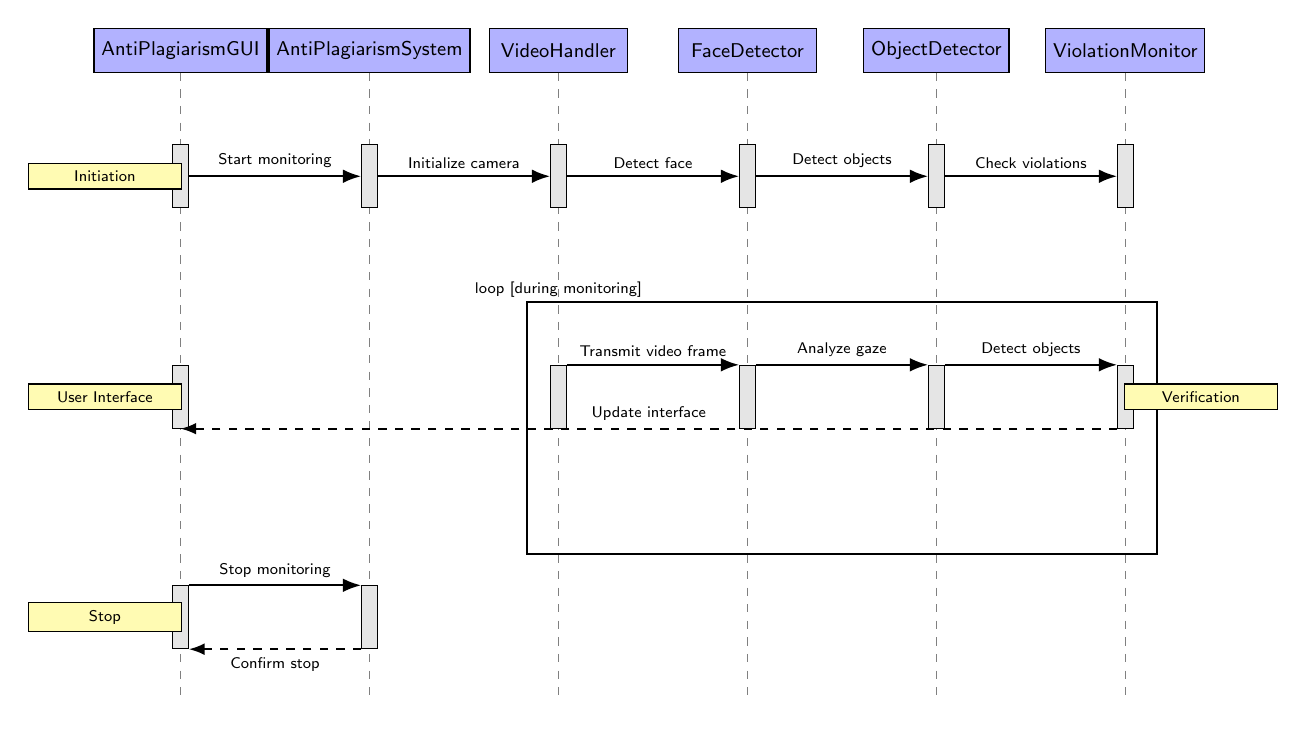
\begin{tikzpicture}[
                scale=0.8,
                transform shape,
                participant/.style={rectangle, draw=black, fill=blue!30, text centered, minimum width=2.2cm, minimum height=0.7cm, font=\sffamily\small},
                activation/.style={rectangle, draw=black, fill=gray!30, minimum width=0.25cm},
                lifeline/.style={dashed},
                message/.style={-{Latex}, thick},
                return/.style={-{Latex[length=2mm]}, dashed, thick},
                note/.style={rectangle, draw=black, fill=yellow!30, text width=2.2cm, text centered, font=\sffamily\scriptsize}
                ]
                % Participants - horizontal alignment with reduced spacing
                \node[participant] (gui) at (0,0) {AntiPlagiarismGUI};
                \node[participant] (sistem) at (3,0) {AntiPlagiarismSystem};
                \node[participant] (video) at (6,0) {VideoHandler};
                \node[participant] (face) at (9,0) {FaceDetector};
                \node[participant] (object) at (12,0) {ObjectDetector};
                \node[participant] (violation) at (15,0) {ViolationMonitor};
                
                % Lifelines
                \draw[lifeline, gray] (gui.south) -- +(0,-10);
                \draw[lifeline, gray] (sistem.south) -- +(0,-10);
                \draw[lifeline, gray] (video.south) -- +(0,-10);
                \draw[lifeline, gray] (face.south) -- +(0,-10);
                \draw[lifeline, gray] (object.south) -- +(0,-10);
                \draw[lifeline, gray] (violation.south) -- +(0,-10);
                
                % Initial activation bars
                \node[activation, fill=gray!20] (gui_act1) at (0,-2) [minimum height=1cm] {};
                \node[activation, fill=gray!20] (sistem_act1) at (3,-2) [minimum height=1cm] {};
                \node[activation, fill=gray!20] (video_act1) at (6,-2) [minimum height=1cm] {};
                \node[activation, fill=gray!20] (face_act1) at (9,-2) [minimum height=1cm] {};
                \node[activation, fill=gray!20] (object_act1) at (12,-2) [minimum height=1cm] {};
                \node[activation, fill=gray!20] (violation_act1) at (15,-2) [minimum height=1cm] {};
                
                % Initial messages
                \draw[message] (gui_act1) -- node[above, font=\sffamily\scriptsize] {Start monitoring} (sistem_act1);
                \draw[message] (sistem_act1) -- node[above, font=\sffamily\scriptsize] {Initialize camera} (video_act1);
                \draw[message] (video_act1) -- node[above, font=\sffamily\scriptsize] {Detect face} (face_act1);
                \draw[message] (face_act1) -- node[above, font=\sffamily\scriptsize] {Detect objects} (object_act1);
                \draw[message] (object_act1) -- node[above, font=\sffamily\scriptsize] {Check violations} (violation_act1);
                
                % Processing loop
                \draw[thick] (5.5,-4) rectangle (15.5,-8);
                \node[font=\sffamily\scriptsize] at (6,-3.8) {loop [during monitoring]};
                
                % Activations in loop
                \node[activation, fill=gray!20] (video_act2) at (6,-5.5) [minimum height=1cm] {};
                \node[activation, fill=gray!20] (face_act2) at (9,-5.5) [minimum height=1cm] {};
                \node[activation, fill=gray!20] (object_act2) at (12,-5.5) [minimum height=1cm] {};
                \node[activation, fill=gray!20] (violation_act2) at (15,-5.5) [minimum height=1cm] {};
                \node[activation, fill=gray!20] (gui_act2) at (0,-5.5) [minimum height=1cm] {};

                % Messages in loop
                \draw[message] (video_act2.north east) -- node[above, font=\sffamily\scriptsize] {Transmit video frame} (face_act2.north west);
                \draw[message] (face_act2.north east) -- node[above, font=\sffamily\scriptsize] {Analyze gaze} (object_act2.north west);
                \draw[message] (object_act2.north east) -- node[above, font=\sffamily\scriptsize] {Detect objects} (violation_act2.north west);
                \draw[return] (violation_act2.south west) -- node[above, font=\sffamily\scriptsize] {Update interface} (gui_act2.south);
                
                % Stop sequence
                \node[activation, fill=gray!20] (gui_act3) at (0,-9) [minimum height=1cm] {};
                \node[activation, fill=gray!20] (sistem_act2) at (3,-9) [minimum height=1cm] {};
                \draw[message] (gui_act3.north east) -- node[above, font=\sffamily\scriptsize] {Stop monitoring} (sistem_act2.north west);
                \draw[return] (sistem_act2.south west) -- node[below, font=\sffamily\scriptsize] {Confirm stop} (gui_act3.south east);
                
                % Explanatory notes - reduced and repositioned
                \node[note] at (-1.2,-2) {Initiation};
                \node[note] at (16.2,-5.5) {Verification};
                \node[note] at (-1.2,-5.5) {User Interface};
                \node[note] at (-1.2,-9) {Stop};
                
                \end{tikzpicture}
                \caption{Sequence diagram of the Anti-Plagiarism system}
        \end{figure}

The sequence diagram illustrates the temporal interaction between the main components of the anti-plagiarism system. The sequence begins when the user initiates monitoring through the \texttt{AntiPlagiarismGUI} interface, which transmits the command to \texttt{AntiPlagiarismSystem}. This, in turn, initializes the camera through \texttt{VideoHandler} and starts the facial detection, object detection and violation monitoring processes.

The main processing loop, highlighted in the diagram, shows how \texttt{VideoHandler} captures video frames which are then analyzed by \texttt{FaceDetector} for face position and gaze direction, followed by \texttt{ObjectDetector} for identifying forbidden objects. \texttt{ViolationMonitor} receives the results of both analyses and determines if there are violations, and the graphical interface is updated accordingly with the new information.

The sequence ends with stopping monitoring, when the user sends the stop command through the interface, and the system confirms the end of the monitoring process. This succession of messages and activations illustrates the complete flow of control and data in the system, from initiation to conclusion, highlighting how all components collaborate to achieve real-time candidate monitoring.

\subsection{Activity diagram}

\begin{figure}[H]
    \centering
    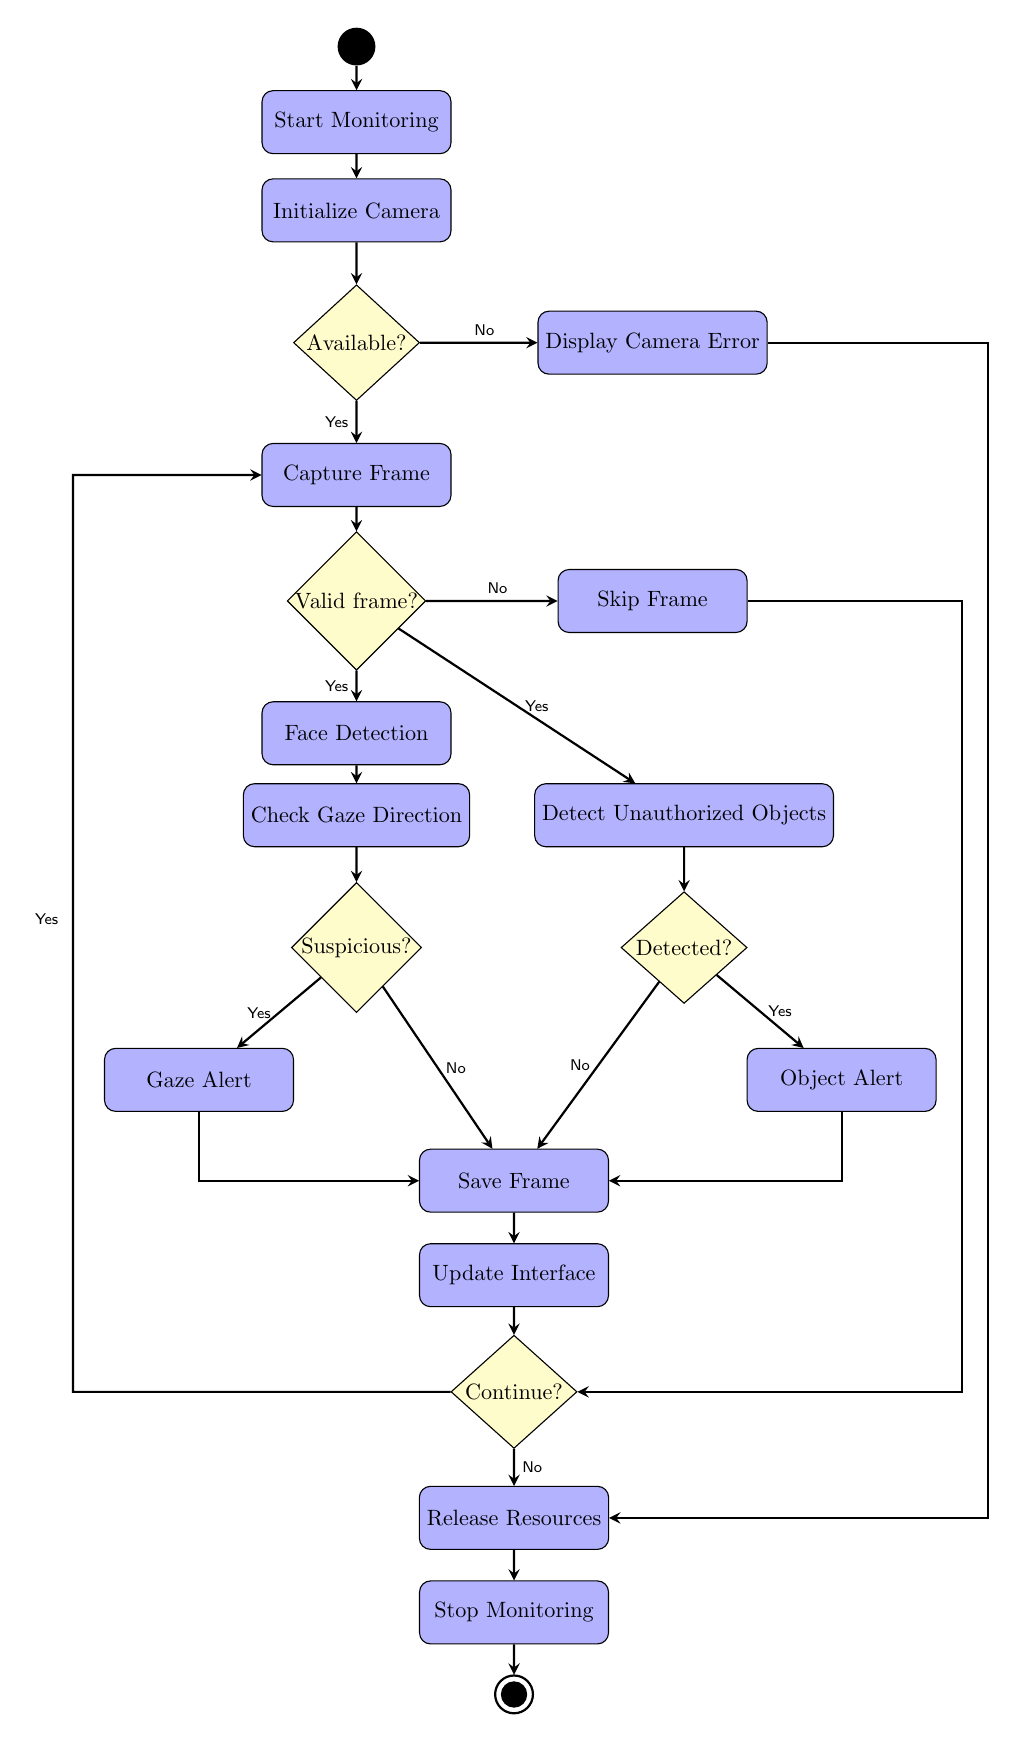
\begin{tikzpicture}[
        scale=0.8,
        transform shape,
        node distance=1.2cm,
        % Node styles
        start/.style={circle, fill=black, minimum width=0.6cm},
        end/.style={circle, draw=black, thick, fill=white, minimum width=0.6cm},
        process/.style={rectangle, draw=black, fill=blue!30, minimum width=3cm, 
                        minimum height=1cm, text centered, rounded corners},
        decision/.style={diamond, draw=black, fill=yellow!20, text centered, 
                        minimum width=2cm, minimum height=0.8cm, inner sep=0pt},
        arrow/.style={thick, ->, >=stealth}
    ]
        % Initial point and nodes
        \node[start] (initpoint) {};
        \node[process, below of=initpoint] (start) {Start Monitoring};
        \node[process, below of=start, yshift=-0.2cm] (init) {Initialize Camera};
        
        % New decision nodes for camera and frame validation
        \node[decision, below of=init, yshift=-0.9cm] (cameracheck) {Available?};
        \node[process, right of=cameracheck, xshift=3.5cm] (errorcamera) {Display Camera Error};
        
        \node[process, below of=cameracheck, yshift=-0.9cm] (capture) {Capture Frame};
        \node[decision, below of=capture, yshift=-0.8cm] (framecheck) {Valid frame?};
        \node[process, right of=framecheck, xshift=3.5cm] (errorframe) {Skip Frame};
        
        % Continue with original flow
        \node[process, below of=framecheck, yshift=-0.9cm] (face) {Face Detection};
        
        % Split into two separate processes
        \node[process, below of=face, yshift=-0.1cm] (gazecheck) {Check Gaze Direction};
        \node[process, right of=gazecheck, xshift=4.0cm] (objectcheck) {Detect Unauthorized Objects};
        
        % Separate decision nodes
        \node[decision, below of=gazecheck, yshift=-0.9cm] (gazeviolation) {Suspicious?};
        \node[decision, below of=objectcheck, yshift=-0.9cm] (objectviolation) {Detected?};
        
        % Separate alerts
        \node[process, below of=gazeviolation, xshift=-2.5cm, yshift=-0.9cm] (gazealert) {Gaze Alert};
        \node[process, below of=objectviolation, xshift=2.5cm, yshift=-0.9cm] (objectalert) {Object Alert};
        
        % Continue flow
        \node[process, below of=gazeviolation, yshift=-2.5cm, xshift = 2.5cm] (save) {Save Frame};
        \node[process, below of=save, yshift = -0.3cm] (update) {Update Interface};
        \node[decision, below of=update, yshift=-0.65cm] (continue) {Continue?};
        \node[process, below of=continue, yshift=-0.8cm] (cleanup) {Release Resources};
        \node[process, below of=cleanup, yshift=-0.3cm] (stop) {Stop Monitoring};
        
        % Draw end node with explicit inner black circle
        \node[end, below of=stop, yshift=-0.1cm] (endnode) {};
        \filldraw[black] (endnode.center) circle (0.2cm);
        
        % Arrows for initial flow
        \draw[arrow] (initpoint) -- (start);
        \draw[arrow] (start) -- (init);
        \draw[arrow] (init) -- (cameracheck);
        
        % Camera check paths
        \draw[arrow] (cameracheck) -- node[right, xshift=-0.2cm, yshift=+0.2cm, font=\sffamily\scriptsize] {No} (errorcamera);
        \draw[arrow] (cameracheck) -- node[left, font=\sffamily\scriptsize] {Yes} (capture);
        \draw[arrow] (errorcamera.east) -- ++(3.5,0) |- (cleanup.east);
        
        % Frame check paths
        \draw[arrow] (capture) -- (framecheck);
        \draw[arrow] (framecheck) -- node[right, xshift=-0.2cm, yshift=+0.2cm, font=\sffamily\scriptsize] {No} (errorframe);
        \draw[arrow] (framecheck) -- node[left, font=\sffamily\scriptsize] {Yes} (face);
        \draw[arrow] (framecheck) -- node[right, font=\sffamily\scriptsize] {Yes} (objectcheck);
        \draw[arrow] (errorframe.east) -- ++(3.4,0) |- (continue.east);
        
        % Split path to two processes
        \draw[arrow] (face) -- (gazecheck);  
        
        % Decision paths
        \draw[arrow] (gazecheck) -- (gazeviolation);
        \draw[arrow] (objectcheck) -- (objectviolation);
        
        \draw[arrow] (gazeviolation) -- node[left, font=\sffamily\scriptsize] {Yes} (gazealert);
        \draw[arrow] (objectviolation) -- node[right, font=\sffamily\scriptsize] {Yes} (objectalert);
        
        % Join paths back
        \draw[arrow] (gazeviolation) -- node[right, font=\sffamily\scriptsize] {No} (save);
        \draw[arrow] (objectviolation) --node[left, font=\sffamily\scriptsize] {No} (save);
        \draw[arrow] (gazealert) |- (save);
        \draw[arrow] (objectalert) |- (save);
        
        % Continue flow
        \draw[arrow] (save) -- (update);
        \draw[arrow] (update) -- (continue);
        \draw[arrow] (continue) -- node[right, font=\sffamily\scriptsize] {No} (cleanup);
        \draw[arrow] (cleanup) -- (stop);
        \draw[arrow] (stop) -- (endnode);
        
        % Loop back to capture
        \draw[arrow] (continue) -- node[left, xshift=-3.1cm, yshift=7.5cm, font=\sffamily\scriptsize] {Yes} ++(-7,0) |- (capture.west);
    \end{tikzpicture}
    \caption{Activity diagram of the Anti-Plagiarism system}
\end{figure}

The activity diagram presents the operational flow of the system, highlighting processing steps and decision points. From the initial state \texttt{Start Monitoring}, activated when the user presses the corresponding button, the system moves to \texttt{Initialize Camera}, where it configures capture parameters and checks webcam availability. This transition corresponds to calling the \texttt{toggle\_monitoring()} method from the main \texttt{AntiPlagiarismGUI} class.

After initialization, the system checks if the respective camera is available through the \texttt{Available?} decision point. In case of an error, the system displays an error message through the \texttt{Display Camera Error} process and advances directly to resource release. This verification is implemented in the \texttt{VideoProcessingThread.run()} method, where the webcam connection is tested.

If it is functional, the process continues with \texttt{Capture Frame}, where frames are captured from the webcam. The system then validates each captured frame through the \texttt{Valid frame?} decision, which checks if the image was obtained correctly. Invalid frames are handled through the \texttt{Skip Frame} process, which ignores them and continues the flow. This verification is implemented through the \texttt{if ret and frame is not None} condition from the video processing module.

After frame validation, the analysis branches into two independent parallel flows:

1. In the first flow, the system executes \texttt{Face Detection}, where \texttt{FaceDetector} locates the candidate's face in the image, followed by \texttt{Check Gaze Direction}, which analyzes the actual position of pupils to determine which direction the candidate is looking, using the \texttt{face\_detector.detect\_direction()} method. At the \texttt{Suspicious?} decision point, it is evaluated whether the gaze direction indicates suspicious behavior (lateral or downward gaze).

2. In parallel, in the second flow, \texttt{Detect Unauthorized Objects} uses YOLOv8 models to scan the image and identify phones or smart watches through the \texttt{object\_detector.detect\_objects()} method. The \texttt{Detected?} decision checks the presence of these forbidden objects.

These two flows operate completely independently, processing the same valid frame but analyzing different aspects - one focusing on candidate behavior and the other on the surrounding environment. This parallelization reflects the modular architecture of the system, where \texttt{FaceDetector} and \texttt{ObjectDetector} function as separate modules.

Each flow can generate specific alerts when detecting potential violations: \texttt{Gaze Alert} for suspicious gazes and \texttt{Object Alert} for unauthorized objects. These are implemented through calling the \texttt{violation\_monitor.log\_violation()} method, which records the details of each violation.

The flows then converge at the \texttt{Save Frame} activity, where the system stores the processed image, followed by \texttt{Update Interface}, which refreshes the display with the analyzed data. This update is performed through the \texttt{frame\_ready} signal from PyQt5, which triggers the graphical interface update.

At the \texttt{Continue?} decision point, the system evaluates whether monitoring should continue. If affirmative, the process returns to \texttt{Capture Frame} for a new iteration. If negative, the system moves to \texttt{Release Resources}, where camera connections are closed and memory is freed, followed by \texttt{Stop Monitoring}, when the process officially ends.

This robust architecture, with parallel processing, allows the system to simultaneously analyze different aspects of the examination situation, increasing efficiency and precision in detecting fraud attempts, even when one of the analysis methods (face or object detection) might encounter temporary difficulties.

\section{Actual Implementation}

In implementing the anti-plagiarism system, it was necessary to use several specialized libraries, each having a different role in its operation.

\subsection{OpenCV}
I used the OpenCV library (\texttt{Open Source Computer Vision Library}),
which had a main role in image processing and analysis\cite{hasan2021face}. With
its help, I captured the video stream from the webcam, through the
\texttt{VideoCapture} function, which acts as the primary interface with the physical
world, capturing images of the candidate which are then analyzed to
detect suspicious behavior.

This library provided me with the \texttt{cvtColor} function, with which I managed to
transform color images into grayscale, which led to much higher efficiency
on the facial detection side, because it reduces
computational complexity, referring only to a single value
for each pixel, instead of three, and improves the performance
of image analysis algorithms, which often work better with
grayscale images.

In the context of precise pupil detection, I applied a Gaussian filter,
with the purpose of reducing noise in images, calling the
\texttt{cv2.GaussianBlur} function, offered by the respective library, which is an
essential filter in image processing. The parameters of this function are
the source image, being the isolated region of the eye, the
kernel size, in our case being 7x7, because it was found, after
several tests, that it offers the best results for pupil detection
and is large enough to cover minor intensity variations
around the pupil, compared to smaller kernels
of 3x3 or 5x5, which preserve too many fine details and noise or
kernels too large of 9x9 or 11x11, which blur the image too much,
leading to loss of the pupil edge and the standard deviation of
the Gaussian distribution, this parameter being set to the value 0,
meaning it is calculated automatically, using the formula:

\begin{equation}
\sigma = 0.3 \cdot \left( \frac{\texttt{kernel\_size} - 1}{2} - 1 \right) + 0.8
\end{equation}

For a kernel of size \(7 \times 7\), this formula becomes:
\begin{align}
\sigma &= 0.3 \cdot \left( \frac{7 - 1}{2} - 1 \right) + 0.8 \nonumber \\
    &= 0.3 \cdot (3 - 1) + 0.8 \nonumber \\
    &= 0.3 \cdot 2 + 0.8 \nonumber = 1.4
\end{align}

The \texttt{cv2.minMaxLoc} function from OpenCV is an essential tool for
pupil detection. This function identifies minimum and maximum values
in an image, along with their coordinates. It returns four
values: the minimum value, the maximum value, the coordinates of the minimum value and
the coordinates of the maximum value. In our case, the value of interest is
represented by the coordinates of the minimum value, because it represents the
darkest point in the eye region, and the pupil is typically the
darkest part of the eye, so this efficient approach allows
rapid localization of the pupil center. This method works
because, before applying \texttt{minMaxLoc}, the image is pre-processed by
that Gaussian filter, mentioned above, which reduces noise and
uniformizes values, making detection more robust to minor variations
in illumination or iris texture.

\begin{figure}[H]
    \centering
    \includegraphics[width=0.5\textwidth]{screenshots/s5.png}
    \caption{RGB values of pixels in the ocular area}
    \label{fig:rgb_ochi}
\end{figure}

The image above represents a screenshot of the RGB values of
pixels in my own ocular area, and these results were obtained with the help of running the test file \texttt{test\_camera.py}.

Also with the help of OpenCV, I managed to draw suggestive visual
elements, such as rectangles in the area of detected objects,
using the \texttt{cv2.rectangle()} function, and to display text for alerts,
using \texttt{cv2.putText()}, and the saving and compression of recordings was
performed using \texttt{VideoWriter}.

Also, I managed to create a mask, to isolate the object of
interest, like the eye, using functions like \texttt{fillPoly} and
\texttt{bitwise\_not}. The \texttt{cv2.fillPoly} function fills a polygonal area in an image
with a specific color, and, in the context of this system, it is used
to create a mask for isolating the eye region. It receives as
parameters the image on which it draws, an array of points that
define the polygon, in our case being the eye contour, and
the fill color, for example (0, 0, 0), which in RGB means
black color. Thus, the result is a mask in which the eye region
is colored black, and the rest of the image remains white.

The \texttt{cv2.bitwise\_not} function inverts the bit values of each pixel
in the image, being equivalent to the bitwise negation operation ($\sim$). I
used it to invert the created mask, so that the eye region
is isolated from the rest of the image. This function receives as
parameters the source image and an optional mask that determines on what
region the operation is applied. Thus, these two functions work
together to create a precise "cut" of the eye region, from
the entire image, to analyze the pupil very precisely, without
interference from other parts of the image.

The \texttt{cv2.circle} function from OpenCV draws a circle on an image, thus I
use it for visual highlighting of detected pupils. I mark the position
of detected pupils on the image, highlight them
using different colors to indicate the state, such as green for
centered gaze or red for suspicious gaze, and provide at the same
time visual feedback for the supervisor, regarding
the candidate's gaze direction. As parameters, the function receives
the image on which the respective circle is drawn, the coordinates of the circle
center, in our case the pupil center, the circle radius, the color
and line thickness, but, for thickness, I used the value -1,
because I wanted a filled circle.

Therefore, the OpenCV library is responsible for everything that means "seeing"
in this system.

\subsection{Dlib}
The Dlib library was used for face detection and facial landmark extraction\cite{el2023drowsiness}. This was essential for gaze analysis and determining its direction.

The \texttt{dlib.get\_frontal\_face\_detector} function was used to initialize the HOG (Histogram of Oriented Gradients) based face detector, which proved efficient even in variable lighting conditions. This algorithm works by dividing the image into small cells and calculating the intensity gradient for each cell. The gradient is then normalized to reduce the effects of illumination variations, and the result is a robust descriptor that can be used to detect faces in the image. The detector returns the coordinates of rectangles that frame the detected faces, and these coordinates are used to isolate the face region.

The facial landmark predictor was loaded using the \texttt{dlib.shape\_predictor} function, which allowed identification of the 68 points on the face. This predictor uses a pre-trained regression-based model, which estimates facial point positions based on features extracted from the image. Among the 68 points, points 36-47 were used to isolate the eye region. These points are distributed to frame the eye contour, allowing precise isolation of the region of interest.

The \texttt{shape.part} function was used to access the coordinates of each facial point, and these coordinates were used to calculate horizontal and vertical gaze ratios. For example, the horizontal ratio is calculated as the ratio between the distance between pupils and the width of the eyes, and the vertical ratio is calculated as the ratio between the height of the eyes and their width. These ratios are used to determine gaze direction, such as looking left, right, up or down.

Also, these points were used to determine head orientation, by calculating distances between key points, such as eyes, nose and mouth. Head orientation is estimated by comparing these distances with reference values, and the result is used to detect head movements that may indicate suspicious behavior.

\subsection{PyTorch and YOLOv8}
For detecting forbidden objects, such as mobile phones and smart watches, I used the PyTorch library\cite{pytorch} and the YOLOv8 model developed by Ultralytics\cite{ultralytics}.

The choice of the YOLO algorithm for this project is based on recent academic research that 
emphasizes that "YOLO is adopted in various applications mainly due to its faster 
inference"\cite{wang2022object}, making it ideal for real-time applications like this prototype. 
This algorithm "uses a simple deep convolutional neural network to detect objects 
in images"\cite{v7labs2023yolo}, making it suitable for real-time detection of objects like 
phones or smart watches, even in variable lighting conditions.

The \texttt{torch.load} function was used to load pre-trained YOLOv8 models. These models are based on the YOLO (You Only Look Once) architecture, which is optimized for fast and precise object detection in images\cite{redmon2018yolov3}. YOLOv8 uses a convolutional neural network that divides the image into grids and simultaneously predicts object classes and their coordinates. This approach enables real-time detection, even on devices with limited resources.

The \texttt{model.predict} method was used to detect objects in the video frame. The model was configured to process only one frame out of 20 to save resources and to detect only categories of interest. This optimization significantly reduces processor and memory consumption, allowing efficient application running on ordinary hardware.

To reduce false positives, I used two separate YOLOv8 models: one for phone detection and another for smart watches. This approach allowed precise classification of detected objects, even in low lighting conditions or when objects were partially visible. For example, the phone model was trained to recognize typical shapes and dimensions of mobile phones, and the smart watch model was trained to detect wearable devices on the wrist.

The \texttt{model.detect} function was used to generate coordinates of detected objects, and these coordinates were used to draw rectangles around objects and to generate real-time alerts. Also, coordinates were used to calculate distances between detected objects and other elements in the image, such as the candidate's face, to determine if objects are actively used.

\subsection{NumPy}
The NumPy library was used for matrix manipulation and numerical data\cite{harris2020array}.

The \texttt{np.zeros} function was used to create masks for regions of interest in the image, and \texttt{np.full} was used to initialize matrices with constant values. These functions are essential for image preprocessing, because they allow isolation of regions of interest and application of specific operations only on these regions\cite{goodfellow2016deep}.

The \texttt{np.min} and \texttt{np.max} functions were used to determine the limits of regions to crop, and vectorial operations allowed rapid calculation of pupil coordinates and horizontal and vertical ratios. For example, pupil coordinates are calculated as points with minimum intensity in the eye region, and ratios are calculated as ratios between distances between these coordinates and region dimensions.

\subsection{Datetime}
The \texttt{datetime}\cite{pythondatetime} library from Python was used for time management and temporal markings in the project. This was essential for event synchronization, report generation and monitoring time recording.

The \texttt{datetime.now()} function was used to obtain the current time at the moment of generating an event, such as detecting an irregularity and saving a report. The created temporal markings are used to link detected events to exact moments in the video stream.

For example, in the \texttt{ViolationMonitor} class, the \texttt{datetime.now().strftime()} function was used to format temporal markings in an easy-to-read format, such as \texttt{YYYY-MM-DD HH:MM:SS}. These are included in generated reports and are used to analyze candidate behavior over time.

The \texttt{timedelta} function was used to calculate time differences between events. For example, the time elapsed since the beginning of recording is calculated using \texttt{datetime.now()} and the recording start time. This is displayed in the graphical interface to provide the user with real-time information about monitoring duration.

Also, the \texttt{datetime} library was used to generate unique names for recording files and reports, using the \texttt{strftime()} function to include temporal markings in file names.

The \texttt{datetime} library was thus an essential tool for time management in all aspects of the project, from real-time monitoring to detailed report generation.

\subsection{Logging}
The \texttt{logging}\cite{pythonlogging} library from Python was used for managing logging messages in the project. This was essential for monitoring application operation, diagnosing problems and maintaining a history of important events.

The \texttt{logging.basicConfig()} function was used to configure the format and logging level. In the project, logging messages are saved both in a file (\texttt{anti\_plagiarism\_system.log}) and displayed in the console. This allows efficient real-time application monitoring, as well as subsequent problem analysis.

For example, in the \texttt{AntiPlagiarismSystem} class, the \texttt{logging} library was used to record important events, such as starting video recording, detecting violations or errors that occurred during processing.

The \texttt{logging} library was also used to record exceptions that occurred during application execution, using the \texttt{logger.exception()} function, which automatically includes exception details in the logging message.

This approach allowed rapid problem identification and application stability improvement. The \texttt{logging} library was thus an essential tool for managing logging messages in all project modules.

\subsection{PyQt5}
For graphical interface development, I used the PyQt5 library\cite{pyqt5}. This allowed creating an intuitive and functional interface, using the following main components:

\begin{itemize}
    \item \textbf{QPushButton:} I used this widget to create interactive buttons, such as those for starting monitoring, recording or exporting reports. These buttons are essential to allow the user to interact with the application in a simple and direct way. For example, the report export button offers clear and accessible functionality for the user.

    \item \textbf{QTextEdit:} This widget is used for real-time display of generated reports. It is a suitable choice because it allows displaying formatted text and can be set as "read-only", so that the user cannot modify the report content.

    \item \textbf{QTimer:} The timer is used for periodic updating of recording time. This is an efficient solution to keep the interface synchronized with background processes, such as real-time monitoring.

    \item \textbf{QLabel:} I used QLabel for displaying important information, such as the number of detected violations or recording time. QLabel is ideal for displaying static or dynamic text, being easy to update depending on application state.

    \item \textbf{QCheckBox:} The checkbox for enabling or disabling image mirroring mode is an intuitive choice. This allows the user to customize how the video stream is displayed, which can be useful depending on their preferences or needs.

    \item \textbf{QGroupBox and Layouts (QVBoxLayout, QHBoxLayout):} These are used for logical organization of interface elements. For example, grouping statistics or controls in a QGroupBox helps create a clearer and more structured interface. Vertical and horizontal layouts are essential for arranging components in a responsive and aesthetic way.

    \item \textbf{QMainWindow:} I used this class as the main window of the application. It is a standard choice for complex applications, because it offers support for menus, toolbars and other advanced elements.

    \item \textbf{QMessageBox:} For displaying confirmation or error messages, QMessageBox is a simple and efficient solution. This allows clear communication with the user at critical moments, such as confirming report export or notifying of an error.
\end{itemize}

The interface was designed to be intuitive and easy to use, offering quick access to all system functionalities.

\subsection{Modularization and project structure}

\hspace{6mm}The project was organized modularly, each Python file having a well-defined role. This approach facilitates code maintenance, testing and functionality extension. Below are detailed the main modules and their responsibilities:

\begin{itemize}
    \item \textbf{main.py:} This is the application entry point. It initializes main components, such as face detector, object detector, violation monitor and video handler. It also manages frame processing and report export.

    \item \textbf{gui\_app.py:} Contains the graphical interface implementation using the PyQt5 library. Includes functionalities such as starting monitoring, video recording, real-time alert display and report export.
    
    \item \textbf{test\_camera.py:} An auxiliary script for testing webcam functionality. Checks if the camera can be accessed and if the video stream is available.

    \item \textbf{modules/face\_detector.py:} This module implements face detection and gaze direction analysis using the Dlib library. It is responsible for face identification and determining the candidate's gaze direction.

    \item \textbf{modules/object\_detector.py:} Contains the implementation for detecting forbidden objects, such as mobile phones and smart watches, using the YOLOv8 model. It is optimized for efficient frame processing.

    \item \textbf{modules/video\_handler.py:} Manages video frame processing and display. Includes functionalities for image mirroring, alert display and saving video recordings.

    \item \textbf{modules/violation\_monitor.py:} Monitors detected violations, such as suspicious gaze or use of forbidden objects. Records alerts and synchronizes them with temporal markings.

    \item \textbf{modules/report\_generator.py:} Is responsible for generating reports in HTML, CSV and JSON formats. These reports include details about detected violations and general statistics.

    \item \textbf{modules/data\_exporter.py:} Manages data export in specified formats (CSV, JSON). It is used to save violation information in a structured way.
    
    \item \textbf{modules/gaze\_tracking/gaze\_tracker.py:} This file implements the main logic for gaze tracking. Uses facial landmarks to calculate horizontal and vertical gaze ratios and to determine its direction.

    \item \textbf{modules/gaze\_tracking/eye.py:} This module isolates the eye region from the image and detects pupils. It also calculates the blinking ratio to identify if the eye is closed.

    \item \textbf{modules/gaze\_tracking/pupil.py:} This file implements the logic for pupil detection and analysis, using their coordinates and dimensions to determine eye state.

    \item \textbf{requirements.txt:} This file contains the list of all libraries and packages needed to run the application. It is used for rapid dependency installation.

    \item \textbf{config.json:} The application configuration file, which stores customizable settings, such as detection thresholds or report saving options.

    \item \textbf{.gitignore:} The file that specifies what files or directories should be ignored by Git, such as temporary files or directories generated when running the program.

    \item \textbf{.devcontainer/:} The directory that contains configuration for the container development environment, which includes Docker files.
\end{itemize}

This modular structure allows clear separation of responsibilities, making the project easier to maintain and extend. Each module can be tested and improved independently, without affecting other parts of the application.

\section{Presentation of usage mode, user interaction and configuration}

This section describes the application usage mode, user interaction and its configuration. Also, screenshots are included to illustrate main functionalities.

\subsection{Usage mode}

To use the application, follow the steps below:
\begin{enumerate}
    \item \textbf{Application launch:} Open the application by running the \texttt{gui\_app.py} file.
    \item \textbf{Initial configuration:} Adjust configuration parameters, such as gaze limits (\textit{left limit}, \textit{right limit}, \textit{down limit}), from the graphical interface or from the \texttt{config.json} file. Also in the \texttt{config.json} file you can modify the confidence threshold for detecting forbidden objects, but it is not recommended, because it is set to a value that ensures the most accurate detection of forbidden objects, due to numerous tests performed.
    \item \textbf{Starting monitoring:} Press the \textbf{Start Monitoring} button to begin video capture and behavior analysis.
    \item \textbf{Starting recording:} Press the \textbf{Start Recording} button to save the video stream and generated alerts.
    \item \textbf{Alert viewing:} Monitor alerts generated in real time in the dedicated section of the interface.
    \item \textbf{Report export:} After session completion, use the \textbf{Export Report} button to save reports in HTML, CSV or JSON format.
\end{enumerate}

\subsection{User interaction}

The application's graphical interface is intuitive and includes the following components:
\begin{itemize}
    \item \textbf{Control buttons:} Allows the user to start/stop monitoring and export reports.
    \item \textbf{Alert section:} Displays real-time alerts generated by the system.
    \item \textbf{Customizable settings:} Offers options for adjusting gaze limit parameters and enabling/disabling image mirroring mode.
    \item \textbf{Stop monitoring:} Press the \textbf{Stop Monitoring} button to stop video capture and behavior analysis.
    \item \textbf{Stop recording:} Press the \textbf{Stop Recording} button to save the video stream and generated alerts in a file.
    \item \textbf{Instant capture:} Press the \textbf{Instant Capture} button to save an image of the current video stream.
\end{itemize}

It will be observed during application use that, depending on gaze direction, the color of the circle drawn on detected pupils will change. For example, if the gaze is centered, the circle will be green, and if the gaze is left, right or down, the circle will be red.

\subsection{Configuration}

The application can be configured by editing the \texttt{config.json} file. Examples of configurable parameters:
\begin{itemize}
    \item \texttt{"left\_limit": 0.7} - Left limit for gaze direction.
    \item \texttt{"right\_limit": 0.3} - Right limit for gaze direction.
    \item \texttt{"down\_limit": 0.6} - Lower limit for gaze direction.
\end{itemize}

\subsection{Screenshots}

\begin{figure}[H]
    \centering
    \includegraphics[width=0.6\textwidth]{screenshots/s1.png}
    \caption{Main application interface}
\end{figure}

\begin{figure}[H]
    \centering
    \includegraphics[width=0.6\textwidth]{screenshots/s2.png}
    \caption{Starting monitoring and recording}
\end{figure}

\begin{figure}[H]
    \centering
    \includegraphics[width=0.6\textwidth]{screenshots/s3.png}
    \caption{Phone detection}
\end{figure}

\begin{figure}[H]
    \centering
    \includegraphics[width=0.6\textwidth]{screenshots/s10.png}
    \caption{Smart watch detection}
\end{figure}

\begin{figure}[H]
    \centering
    \includegraphics[width=0.6\textwidth]{screenshots/s4.png}
    \caption{Report export}
\end{figure}

\section{Personal contribution}

In this project, I brought several significant contributions, which include:

\subsection{Using two YOLOv8 models for detecting forbidden objects}
I used two separate YOLOv8 models, one specialized for detecting mobile phones and another for detecting smart watches. This approach was chosen to work efficiently and to eliminate false positives. Instead of retraining a single model for both categories, I applied strict classifications based on the \textit{x-y} dimensions of detected objects. I specify that each YOLOv8 model has a different confidence threshold, and these values were established following certain tests performed and are found in the main configuration file \texttt{config.json}. Thus, \texttt{confidence\_threshold} is set to 0.55 for phones and 0.4 for smart watches. These values are essential to ensure precise detection and to minimize the risk of false positives.

\subsection{Implementation of linear algebra calculations for gaze analysis}
I developed and integrated linear algebra calculations to determine the user's gaze direction. These calculations include:
\begin{itemize}
    \item Determining pupil coordinates using vectors and reference points.
    \item Calculating horizontal and vertical ratios (\textit{horizontal ratio} and \textit{vertical ratio}) to estimate gaze direction.
    \item Filtering and adjusting values to eliminate noise and unexpected variations.
\end{itemize}

The horizontal ratio is essential for determining if the respective candidate is looking left or right. This algorithm calculates the ratio based on pupil positions and includes an adjustment component for head orientation.

\begin{algorithm}[H]
    \caption{Horizontal ratio calculation (X axis - left/right)}
    \begin{algorithmic}[1]
    \Procedure{CalculateHorizontalRatio}{}
        \If{$pupils\_found = false$}
            \State \Return $0.5$ \Comment{Pupils not detected $\implies$ return neutral value}
        \EndIf
    
        \State $left\_pupil\_pos \gets \frac{left\_pupil.x}{(left\_eye\_center.x \cdot 2 - 10)}$ \Comment{Normalize X position}
        \State $right\_pupil\_pos \gets \frac{right\_pupil.x}{(right\_eye\_center.x \cdot 2 - 10)}$
        \State $pupil\_ratio \gets \frac{left\_pupil\_pos + right\_pupil\_pos}{2}$ \Comment{Average of normalized positions}
    
        \If{$left\_origin \neq null$ \textbf{and} $right\_origin \neq null$}
            \State $left\_abs\_center \gets left\_origin.x + left\_eye\_center.x$
            \State $right\_abs\_center \gets right\_origin.x + right\_eye\_center.x$
            \State $eye\_distance \gets right\_abs\_center - left\_abs\_center$
    
            \If{$frame \neq null$}
                \State $frame\_width \gets frame.shape[1]$ \Comment{Actual image width}
            \Else
                \State $frame\_width \gets 640$ \Comment{Default value if no frame exists}
            \EndIf
    
            \State $position\_factor \gets \frac{eye\_distance}{frame\_width \cdot 0.3}$ \Comment{Evaluate relative head position}
            \State $adjusted\_ratio \gets pupil\_ratio$ \Comment{Initially, ratio is not modified}
    
            \If{$position\_factor < 0.8$}
                \State $adjusted\_ratio \gets \max(0.6, pupil\_ratio)$ \Comment{Head turned left}
            \ElsIf{$position\_factor > 1.2$}
                \State $adjusted\_ratio \gets \min(0.4, pupil\_ratio)$ \Comment{Head turned right}
            \EndIf
    
            \State \Return $adjusted\_ratio$
        \EndIf
    
        \State \Return $pupil\_ratio$ \Comment{No head data $\implies$ return direct average}
    \EndProcedure
    \end{algorithmic}
    \end{algorithm}
    
The vertical ratio is used to determine if the candidate's gaze is oriented downward. This algorithm calculates the ratio based on vertical pupil positions and includes an adjustment component for head inclination.

\begin{algorithm}[H]
    \caption{Vertical ratio calculation (Y axis - up/down)}
    \begin{algorithmic}[1]
    \Procedure{CalculateVerticalRatio}{}
        \If{$pupils\_found = false$}
            \State \Return $0.5$ \Comment{Cannot estimate direction $\implies$ default value}
        \EndIf
    
        \State $left\_pupil\_pos \gets \frac{left\_pupil.y}{(left\_eye\_center.y \cdot 2 - 10)}$ \Comment{Normalize Y position}
        \State $right\_pupil\_pos \gets \frac{right\_pupil.y}{(right\_eye\_center.y \cdot 2 - 10)}$
        \State $pupil\_ratio \gets \frac{left\_pupil\_pos + right\_pupil\_pos}{2}$ \Comment{Average of normalized positions}
    
        \If{$left\_origin \neq null$ \textbf{and} $right\_origin \neq null$}
            \State$eye\_center\_y \gets \frac{left\_origin.y + left\_eye\_center.y + right\_origin.y + right\_eye\_center.y}{2}$
            \State$mouth\_pos \gets left\_origin.y + left\_eye\_center.y + 50$ \Comment{Mouth estimation}
            \State$face\_height \gets |eye\_center\_y - mouth\_pos|$ \Comment{Face height estimation}
    
            \If{$face\_height > 0$}
                \State$position\_factor \gets \frac{|left\_origin.y - eye\_center\_y|}{face\_height}$ \Comment{Head inclination (up/down)}
            \Else
                \State$position\_factor \gets 0.5$ \Comment{Default value when calculation is not valid}
            \EndIf
    
            \State$adjusted\_ratio \gets pupil\_ratio$
    
            \If{$position\_factor > 0.6$}
                \State$adjusted\_ratio \gets \min(0.4, pupil\_ratio)$ \Comment{Head is bent}
            \ElsIf{$position\_factor < 0.4$}
                \State$adjusted\_ratio \gets \max(0.6, pupil\_ratio)$ \Comment{Head is raised}
            \EndIf
    
            \State\Return$adjusted\_ratio$
        \EndIf

        \State\Return$pupil\_ratio$ \Comment{Incomplete data $\implies$ return initial average}
    \EndProcedure
    \end{algorithmic}
    \end{algorithm}
    
These algorithms work together to create a robust gaze direction detection system. The calculated ratios are compared with predefined thresholds to determine if the candidate is looking center, left, right or down, and the results of this analysis are used to generate corresponding alerts.

This implementation offers several significant advantages:

\begin{enumerate}
    \item \textbf{Robustness to illumination variations} - By using the minimum point method for pupil detection, the algorithm is less sensitive to lighting changes.
    
    \item \textbf{Head orientation compensation} - The adjustments implemented for the eye position factor and head inclination factor allow distinguishing between a suspicious gaze and natural head movement.
    
    \item \textbf{Coordinate normalization} - Converting absolute coordinates to normalized ratios makes the algorithm adaptable to different camera resolutions and distances from the screen.
    
    \item \textbf{Optimized threshold-based filtering} - The thresholds used were determined empirically to offer the best balance between detection rate and false positive rate.
\end{enumerate}

These algorithms have been tested in various lighting conditions, demonstrating high accuracy in gaze direction detection, thus contributing to the efficiency of the anti-plagiarism system.

\subsection{Real-time video processing optimization}
I implemented video processing optimizations, considering that the human mind cannot instantly process certain information that can be used for exam fraud purposes, including:
\begin{itemize}
    \item Processing one frame out of 30 for object detection, thus reducing resource consumption.
    \item Using a circular buffer for efficient video frame management.
    \item Integrating a cache system for generated alerts, avoiding duplication of alert messages.
\end{itemize}

\subsection{Detailed report generation}
I developed an automatic report generation system in HTML, CSV and JSON formats. These reports include:
\begin{itemize}
    \item The exact time of each detected violation.
    \item The type of detected object and its location in the video frame.
    \item General summary of the monitoring session.
\end{itemize}

\begin{figure}[H]
    \centering
    \includegraphics[width=0.6\textwidth]{screenshots/s11.png}
    \caption{Example report generated in HTML format} 
\end{figure}

\subsection{Intuitive graphical interface integration}
I developed an intuitive graphical interface using PyQt5, which allows users to:
\begin{itemize}
    \item Start and stop real-time monitoring.
    \item View alerts generated in real time.
    \item Export detailed reports with a single click.
\end{itemize}

\subsection{Real-time gaze limit parameter editing}
I implemented a functionality that allows the user to edit gaze limit parameters (\textit{left limit}, \textit{right limit}, \textit{down limit}) in real time, without requiring application restart. This functionality is useful in particular scenarios, such as differences between taking an exam on computer and on paper. 

For example, in the case of a paper exam, the candidate is forced to bend more to write, which can reduce the false positive rate by adjusting the lower limit (\textit{down limit}). This flexibility offers supervisors the possibility to quickly adapt the system to the specific context of the exam.

This functionality contributes to reducing false positives and increasing system accuracy in certain frequently encountered scenarios.

\section{Difficulties encountered}

In realizing this project, I encountered several difficulties, in which I used certain constraints and less conventional solutions, to have results as close as possible to those desired:

\begin{enumerate}
    \item \textbf{YOLOv8 model integration:} Configuring and optimizing YOLOv8 models for detecting forbidden objects was a challenge, especially regarding reducing false positives. It was necessary to adjust detection thresholds and use separate models for different object categories.

    \item \textbf{Performance on limited hardware:} Real-time video processing was difficult on devices with limited hardware resources. I implemented optimizations, such as processing one frame out of 30 and using a circular buffer, to reduce resource consumption.

    \item \textbf{Gaze detection in variable lighting conditions:} Precise gaze direction detection was affected by lighting variations. It was necessary to apply filters and adjust algorithm parameters to improve robustness.

    \item \textbf{Multimedia data synchronization:} Precise correlation between video, audio stream and detected events was a complex task. I used synchronized temporal markings to link alerts generated by exact moments in the video stream.

    \item \textbf{Graphical interface complexity:} Developing an intuitive and functional graphical interface was a challenge, especially regarding logical organization of components and their synchronization with background processes.

    \item \textbf{False positive management:} During testing, I observed a high rate of false positives, especially in object detection. It was necessary to adjust algorithms and implement additional filters to improve accuracy.

    \item \textbf{Code documentation and modularization:} Structuring the project in a modular way and clear documentation of each module required additional time, but were essential for maintenance and subsequent application extension.

    \item \textbf{Testing and validation:} Testing the application in real scenarios was difficult, especially in simulating varied usage conditions, such as different camera angles, poor lighting or background noise.

    \item \textbf{Dependency management:} Correct installation and configuration of all necessary libraries and packages were sometimes problematic, especially due to incompatibilities between versions.
\end{enumerate}

\section{Conclusions}

The \textit{Anti-Plagiarism Monitoring System for Exams} project successfully achieved the proposed objectives, offering an innovative and efficient solution for monitoring candidate behavior during exams. 

\subsection{Objective fulfillment}

\begin{itemize}
    \item \textbf{Candidate gaze detection:} The system uses advanced image processing technologies to analyze gaze direction and signal deviations from normal behavior. This functionality was successfully implemented, offering precise and real-time detection.
    
    \item \textbf{Identification of unauthorized objects:} Through integration of YOLOv8 models, the application detects devices such as mobile phones and smart watches, contributing to preventing fraud attempts.
    
    \item \textbf{Recording and archiving:} The system allows recording of exam sessions, offering the possibility to subsequently analyze candidate behavior and archive evidence.
    
    \item \textbf{Report generation:} The application generates detailed reports in HTML, CSV and JSON formats, facilitating analysis and incident documentation.
    
    \item \textbf{Intuitive interface:} The graphical interface developed with PyQt5 is easy to use and offers quick access to all system functionalities.
\end{itemize}

\subsection{Utility and relevance}

Plagiarism and fraud attempts represent major problems in modern educational systems. The proposed application offers a current and relevant solution, using cutting-edge technologies to combat these problems. By focusing on candidates' physical behavior, the system brings a significant advantage compared to existing solutions, which focus mainly on screen activity monitoring.

\subsection{Performance and optimizations}

The system was optimized to function efficiently even on limited hardware, using techniques such as processing one frame out of 30 and reducing resource consumption. Conducted tests demonstrated a high accuracy rate in detecting suspicious behavior and forbidden objects, with a low false positive rate.

\subsection{Impact and relevance}

The application's impact is significant, contributing to maintaining academic integrity and creating a fair exam environment. Through the use of artificial intelligence and image processing technologies, the system can be extended and adapted for various educational and professional contexts.

\subsection{Advantages compared to other similar solutions}

Compared to other existing solutions, our application offers the following advantages:
\begin{itemize}
    \item \textbf{Focus on physical behavior:} Unlike solutions that monitor only screen activity, this system analyzes gaze direction and detects unauthorized objects.
    \item \textbf{Reduced costs:} Local implementation significantly reduces costs per candidate, compared to commercial solutions like ProctorU.
    \item \textbf{Platform independence:} The application functions independently of browser or other platforms, offering increased flexibility.
    \item \textbf{Detailed reports:} Automatic report generation in multiple formats facilitates subsequent analysis and incident documentation.
\end{itemize}

\subsection{Multi-platform compatibility}
Our application runs on both Windows and Linux (Ubuntu), offering users flexibility depending on their preferred operating system. 

On Windows, the application benefits from GPU support through CUDA, which allows using the NVIDIA graphics card for accelerating video processing and object detection. This is possible due to how NVIDIA drivers are stored and managed on Windows.

On Linux, although the application functions correctly, GPU integration through CUDA has not yet been fully implemented. This limitation is due to differences in NVIDIA driver management on Linux compared to Windows. Currently, processing on Linux is performed exclusively on CPU, but implemented optimizations ensure acceptable performance even in these conditions.

This multi-platform compatibility makes the application accessible to a wide spectrum of users, regardless of the operating system used.

\subsection{Possible improvements}

Although the current application offers advanced functionalities for anti-plagiarism monitoring, there are several aspects that can be improved or extended to increase its efficiency and utility:

\begin{enumerate}
    \item \textbf{Integration with LMS platforms:} Adding support for direct integration with learning management systems (LMS), such as Moodle, Blackboard or Canvas, to facilitate exam and report management.

    \item \textbf{Multi-camera support:} Extending the application to allow simultaneous use of multiple cameras, offering a more complete perspective on candidate behavior.

    \item \textbf{Advanced audio monitoring:} Developing a more sophisticated audio processing module, which detects suspicious conversations or use of unauthorized audio devices.

\end{enumerate}

These improvements could significantly increase the application's value and would extend its usage area in various educational and professional contexts.

Recent research in the field of smart watches has proposed "a categorization of smart watch use in the health sector in 3 key functional domains: monitoring, guidance and 
prediction"\cite{moshawrab2023value}, concepts that could be adapted for monitoring 
candidate behavior. Also, studies have demonstrated the efficiency of "smart watch-based frameworks for real-time mobility assessment and monitoring"\cite{kheirkhahan2018smartwatch}, 
suggesting the possibility of integrating these technologies in future versions of this system to 
improve accuracy in detecting suspicious behavior. \cite{brainard2018massive}

In conclusion, the project represents a significant contribution to the anti-plagiarism monitoring field, offering a modern, efficient and adaptable solution to current educational system needs.

\newpage
\printbibliography[heading=bibintoc, title={Bibliography}]

\end{document}